\documentclass[18p]{beamer}
\usetheme{ALUF}
\usepackage[utf8]{inputenc}
% \usepackage{palatino}
% \usepackage[T1]{fontenc}
\usepackage{lmodern}
\usepackage[expert]{mathdesign}
\usepackage[protrusion=true,expansion=true,tracking=true,kerning=true]{microtype}
\setbeamercovered{transparent}

\usepackage[backend=biber]{biblatex}
\addbibresource{main.bib}

\usepackage{graphicx}

% declare the path(s) where your graphic files are
\graphicspath{./img/}
% and their extensions so you won't have to specify these with
% every instance of \includegraphics
\DeclareGraphicsExtensions{.pdf,.jpeg,.png}


\font\myfont=cmr12 at 12pt
\title{\myfont Finite-Time Stabilization-Based \\Adaptive Fuzzy Control Design}
%\subtitle{As if this needs a subtitle}
\author{Prepered for Adaptive Control Project\\ Professor Bagheri}
\date{Summer 2025}
\institute{Presentation \\Murtaza Asaadi}

\begin{document}
\begin{frame}[plain,t]
	\titlepage
\end{frame}

%%%%%%%%%%%%%%%%%%%%%%%%%%%%%%%%%%
\section{Outline}
\begin{frame}% [plain,t]
	\frametitle{Outline}
	\begin{enumerate}
		\item Introduction
		\item Problem Formulation
		\item The Control Strategy
		\item Adaptive Law Design
		\item Stability Analysis
		\item Python Implementation
		\item Simulation Results
		\item Conclusion
	\end{enumerate}
\end{frame}

%%%%%%%%%%%%%%%%%%%%%%%%%%%%%%%%%%
\section{Introduction}
\begin{frame}
	\frametitle{What is the Problem?}
		\begin{itemize}
		\item Controlling nonlinear systems is challenging due to uncertainties and complex dynamics.
		\item Traditional controllers guarantee stability over an infinite time horizon (asymptotic stability).
	\end{itemize}
\end{frame}

\begin{frame}
	\frametitle{Why Finite-Time Control?}
	Many real-world applications (robotics, aerospace) require systems to reach their desired state within a specific, finite time.\\
	\vspace*{2\baselineskip}
	\textbf{Benefits of Finite-Time Stability:}
	\begin{itemize}
		\item Faster convergence rates.
		\item Higher precision in tracking.
		\item Improved robustness against disturbances.
	\end{itemize}
\end{frame}

\begin{frame}
	\frametitle{Contribution}
	\begin{itemize}
	\item Develops an adaptive fuzzy control strategy for a class of nonlinear systems.
	\item Guarantees that the system's tracking error converges to a small region around zero in finite time.
	\item Ensures all signals in the closed-loop system remain bounded and stable.
\end{itemize}
\end{frame}

%%%%%%%%%%%%%%%%%%%%%%%%%%%%%%%%%%
\section{Formulation}
\begin{frame}
	\frametitle{System Representation}
\[
\left\{
\begin{aligned}
	\dot{z}_i &= \phi_i(\bar{z}_i) + \varphi_i(\bar{z}_i) z_{i+1}, \quad i = 1, \ldots, n-1 \\
	\dot{z}_n &= \phi_n(z) + \varphi_n(z) q(v) \\
	y &= z_1
\end{aligned}
\right.
\]

\begin{itemize}
	\item $z_i$: System states.
	\item $\phi_i, \varphi_i$: Unknown nonlinear functions.
	\item $v$: The control input we design.
	\item $q(v)$: A quantizer, which models the digital nature of controllers (discrete signal levels).
	\item $y$: The system output.
\end{itemize}
\end{frame}


\begin{frame}
	\frametitle{Control Objective}
	Design a \textbf{control law $v$} such that the \textbf{system output $y$} follows a desired \textbf{reference signal $y_r$} in finite time, despite the unknown functions and the quantizer.
\end{frame}


%%%%%%%%%%%%%%%%%%%%%%%%%%%%%%%%%%
\section{Control}
\begin{frame}
	\frametitle{Key Components of Control Strategy}
	The controller is designed using a combination of techniques:
	\begin{itemize}
		\item Backstepping
		\item Fuzzy Logic Systems (FLS)
		\item Adaptive Control
		\item Hysteretic Quantizer
	\end{itemize}
\end{frame}
\begin{frame}
	\frametitle{Backstepping}
 A recursive design methodology. It breaks down the complex n-dimensional system into a series of 1-D problems, designing a "virtual controller" at each step.
\end{frame}
\begin{frame}
	\frametitle{Fuzzy Logic Systems}
Used as universal approximators. Since the functions $\phi$ and $\phi_i$ are unknown, an FLS is used to estimate their behavior online.
\end{frame}
\begin{frame}
	\frametitle{Adaptive Control}
The parameters of the Fuzzy Logic System are not fixed; they are "adapted" or tuned in real-time by adaptive laws to improve approximation accuracy.
\end{frame}
\begin{frame}
	\frametitle{Hysteretic Quantizer}
The control input $v$ is passed through a quantizer $q(v)$. This models the constraints of digital hardware and communication channels.
\end{frame}

%%%%%%%%%%%%%%%%%%%%%%%%%%%%%%%%%%
\section{Adaptive}
\begin{frame}
	\frametitle{Controller and Adaptive Law Design}
	The design follows the backstepping procedure, step-by-step.
	\begin{itemize}
		\item Step 1: Virtual Controller $\alpha_1$
		\item Step 2: Actual Controller $v$
		\item Adaptive Laws
	\end{itemize}
\end{frame}
 \begin{frame}[noframenumbering]
 	\frametitle{Controller and Adaptive Law Design}
 	The design follows the backstepping procedure, step-by-step.
 	\begin{itemize}
 		\item Step 1: Virtual Controller $\alpha_1$
 		\begin{itemize}
 			\item Define the first error surface: $\eta_1=z_1-y_r$.
 			\item Design a virtual controller $\alpha_1$ to stabilize this error.
 			\item $\alpha_1$ includes terms to drive the error to zero and a fuzzy logic term to cancel nonlinearities.
 		\end{itemize}
 		\item Step 2: Actual Controller $v$
 		\item Adaptive Laws
 	\end{itemize}
 \end{frame}
 \begin{frame}[noframenumbering]
 	\frametitle{Controller and Adaptive Law Design}
 	The design follows the backstepping procedure, step-by-step.
 	\begin{itemize}
 		\item Step 1: Virtual Controller $\alpha_1$
 		\item Step 2: Actual Controller $v$
 		\begin{itemize}
 			\item Define the final error surface: $\eta_2=z_2-\alpha_1$.
 			\item Design the actual control input $v$ to stabilize $\eta_2$.
 		\end{itemize}
 		\item Adaptive Laws
 	\end{itemize}
 \end{frame}
 \begin{frame}[noframenumbering]
 	\frametitle{Controller and Adaptive Law Design}
 	The design follows the backstepping procedure, step-by-step.
 	\begin{itemize}
 		\item Step 1: Virtual Controller $\alpha_1$
 		\item Step 2: Actual Controller $v$
 		\item Adaptive Laws
 		 \begin{itemize}
 			\item For each fuzzy system, an adaptive law updates its weight parameter $\theta_i$.
 			\item The goal is to minimize the function approximation error.
 		\end{itemize}
 	\end{itemize}
 \end{frame}
%%%%%%%%%%%%%%%%%%%%%%%%%%%%%%%%%%
\section{Stability}
\begin{frame}
	\frametitle{Stability Analysis}
A total Lyapunov function V is constructed for the entire closed-loop system.
The paper proves that the derivative of the Lyapunov function satisfies:
\begin{equation*}
	\dot{V} \le -\lambda_0 V - \lambda_1 V^h + b_0
\end{equation*}

\begin{itemize}
	\item $\lambda_0 V$: Guarantees exponential stability.
	\item $\lambda_1 V^h$: Guarantees finite-time stability.
	\item $b_0$: A small positive constant due to approximation errors.
\end{itemize}
\end{frame}
\begin{frame}
	\frametitle{Theorem 1 (Main Result)}
	The designed controller ensures that:
	\begin{itemize}
		\item The system is practically stable in finite time. The tracking error converges to a small, bounded region around zero.
		\item The size of this region and the convergence time can be calculated.
		\item All signals within the system (states, adaptive parameters) remain bounded.
		\end{itemize}
\end{frame}
%%%%%%%%%%%%%%%%%%%%%%%%%%%%%%%%%%
\section{Python}
\begin{frame}
	\frametitle{Python Implementation Overview}
The simulation was reproduced using Python with SciPy and Matplotlib.\\
\vspace*{1\baselineskip}
\textbf{Key Implementation Steps:}
\begin{itemize}
	\item Define Parameters
	\item Hysteretic Quantizer
	\item Fuzzy Basis Functions
	\item System Model Function
	\item ODE Solver
	\item Plotting
\end{itemize}
\end{frame}

%%%%%%%%%%%%%%%%%%%%%%%%%%%%%%%%%%
\section{Simulation}
\begin{frame}
	\frametitle{System Output vs. Reference Signal}
	\vspace*{1\baselineskip}
			\begin{figure}[h!]
		\centering
		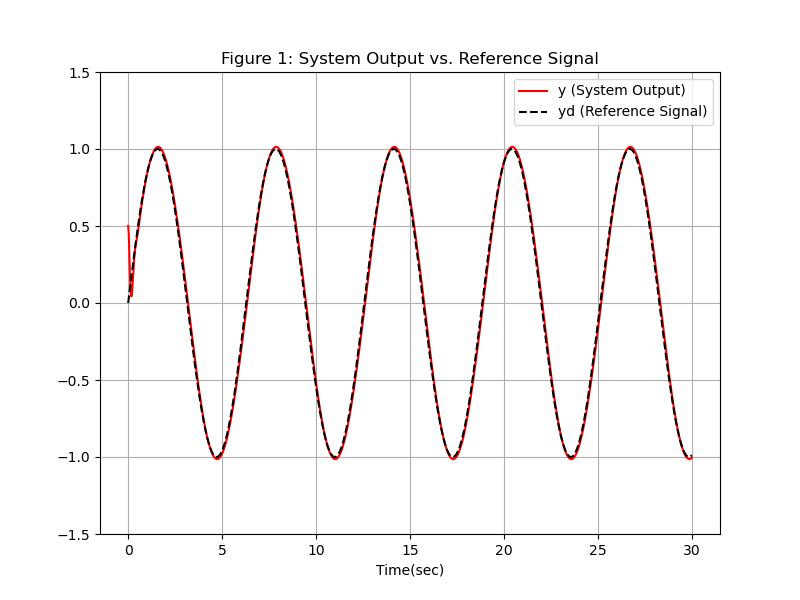
\includegraphics[width=0.70\textwidth]{./img/sim1.png}
	\end{figure}
		\begin{itemize}
		\item The plot shows the system output $y$ quickly converging to and tracking the sinusoidal reference signal $y_d$.
		\item This demonstrates the effectiveness of the tracking control.
	\end{itemize}
\end{frame}
\begin{frame}
	\frametitle{State Variable $z_2$}
	\vspace*{1\baselineskip}
		\begin{figure}[h!]
		\centering
		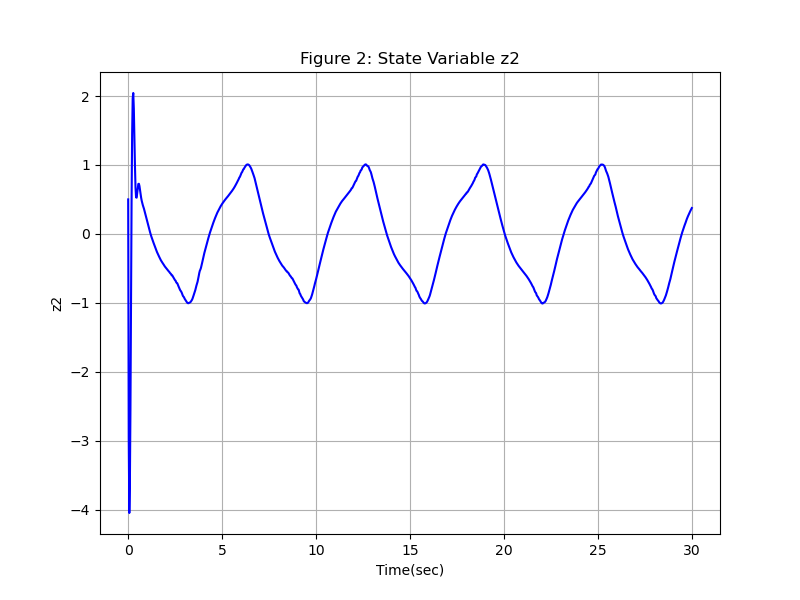
\includegraphics[width=0.70\textwidth]{./img/sim2.png}
	\end{figure}
	\begin{itemize}
		\item The state $z_2$ remains bounded throughout the simulation, confirming the stability of all system signals.
	\end{itemize}
\end{frame}
\begin{frame}
	\frametitle{Adaptive Parameters}
	\vspace*{1\baselineskip}
	\begin{figure}[h!]
		\centering
		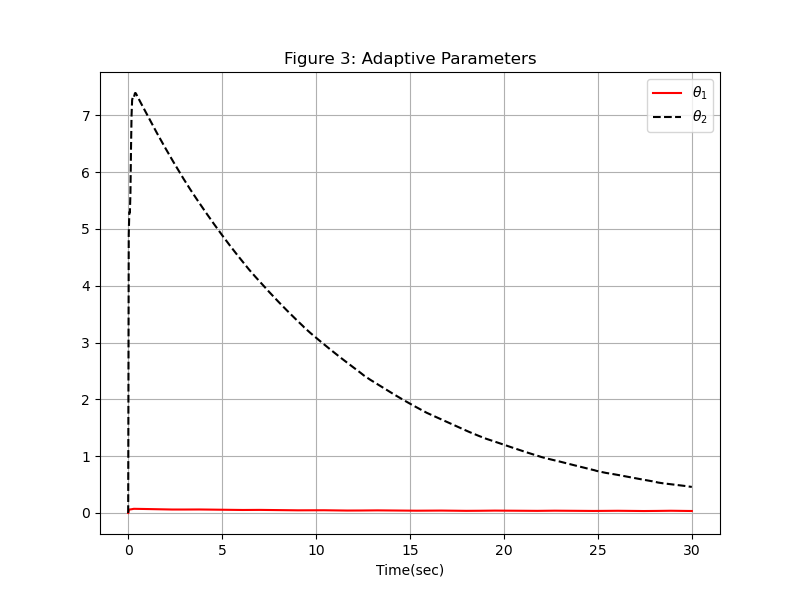
\includegraphics[width=0.70\textwidth]{./img/sim3.png}
	\end{figure}
	\begin{itemize}
		\item The adaptive parameters $\theta_1$ and $\theta_2$ converge to stable values.
\item This indicates that the fuzzy logic systems have successfully learned to approximate the unknown nonlinearities.
	\end{itemize}
\end{frame}
\begin{frame}
	\frametitle{Quantizer Output}
	\vspace*{1\baselineskip}
	\begin{figure}[h!]
		\centering
		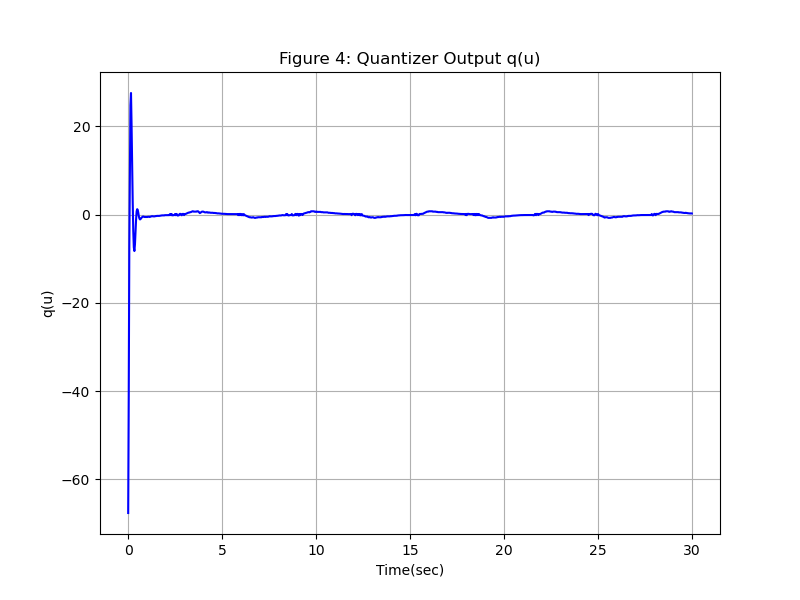
\includegraphics[width=0.70\textwidth]{./img/sim4.png}
	\end{figure}
	\begin{itemize}
		\item This plot shows the discrete output of the hysteretic quantizer.
		\item It highlights that the controller operates effectively even with a non-continuous, quantized input signal.
	\end{itemize}
\end{frame}
%%%%%%%%%%%%%%%%%%%%%%%%%%%%%%%%%%
\section{Conclusion}
\begin{frame}
	\frametitle{Conclusion}
	\begin{itemize}
		\item<1,6> Successfully simulated an adaptive fuzzy controller that achieves finite-time stability for a class of nonlinear systems.
		\item<2,6> The use of backstepping and fuzzy logic systems effectively handles system uncertainties.
		\item<3,6> The design explicitly accounts for input quantization, making it more practical for digital implementation.
		\item<4,6> Stability analysis proves that all signals are bounded and the tracking error converges to a small region in finite time.
		\item<5,6> The Python simulation verifies the theoretical results, showing excellent tracking performance and stability.
	\end{itemize}
\end{frame}



\ThankYouFrame


\end{document}
